\addcontentsline{toc}{subsection}{Applications of Derivatives}
\vbtitle[\Large]{Applications of Derivatives} 

\vbsubtitle{Geometrical Interpretation of Derivative:}

\begin{center}
    \begin{tikzpicture}
    % [thick, scale=3.5]
    % \clip (2, 1) rectangle (4.25, 4);
    \def\tat{3.65}%tangent at {x}
    \def\dx{0.5}%tangent at {x}
        \tzaxes(-0.5, -0.5)(7,4){$x$}{$y$}
        \tztos"curve"
            (0,0)[out=0, in=-180]
            (3,1.5)[out=0, in=-180]
            (6, 3.5);
            
        \tzvXpointat*{curve}{\tat-\dx}(A)
        \tzvXpointat*{curve}{\tat+\dx}(B)
        % \tztangentat"TL"{curve}{\tat}[\tat-1.5:5]
        \tzcoor($($(A)!0.5!(B)$)!1cm!90:(B)$)(O)%{$O$}[ar]
        %\tzXpoint{normal}{normall}(X)
        % \tzcircle[dashed](O)(1)
        % \tzline[dashed, red](O)(A){$r$}[ml]
        % \tzline[dashed, red](O)(B)
        \tzcoor*($(A)+(2*\dx, 0)$)(C)
        \tzline(A)(C){$\Delta x$}[mb]
        \tzline(B)(C){$\Delta y$}[mr]
        \tzline(A)(B){$\Delta l$}[ma]
        \tzLFn(A)(B)[1:5.5]
        % \tzanglemark(C)(A)(B){$\theta$}(5pt)
        % \tzanglemark(B)(O)(A){$d\theta$}(5pt)
    \end{tikzpicture}
\end{center}
\vbdefinition{
    To understand the geometrical meaning, we plotted a curve in the \( xy \) plane. The curve is represented by the equation \( y = f(x) \). We took two different points on the curve and drew a secant line passing through them.\\[2mm] 
    There is a chord length \( \Delta l \) between the two points. Assuming this chord as the hypotenuse, we can draw a right-angled triangle with base \( \Delta x \) and height \( \Delta y \) along the \( x \) and \( y \) axes, respectively. \\[2mm]
    Now, imagine that the two points are getting closer and closer on the curve. The chord length \( \Delta l \) will become smaller and smaller, and hence \( \Delta x \) and \( \Delta y \) will also become smaller.\\[2mm]
    There will be a point where the two points will be so close that the chord length \( \Delta l \) will tend to zero, and the secant line will become a tangent line to the curve at that point.\\[2mm]
    At this point, \( \Delta x \) will also tend to zero. As we know that the slope of the line is given by \( \frac{\Delta y}{\Delta x} \), and \(\underset{\Delta x \to 0}{\lim} \frac{\Delta y}{\Delta x}\) is the derivative of the function at that point. These both are the same when the two points are very close to each other. This means that the derivative of a function at a point is the slope of the tangent line to the curve at that point.
}
\begin{align*}
    \textit{Slope of the secant line } &= \frac{\Delta y}{\Delta x}\\
    \underset{\Delta x \to 0}{\lim}\left(\textit{Slope of the secant line }\right) &= \underset{\Delta x \to 0}{\lim} \frac{\Delta y}{\Delta x} \\
    \Rightarrow \textit{Slope of the tangent line } &= \frac{dy}{dx}\\
    \Aboxed{\frac{dy}{dx} &= \tan \theta }
\end{align*}

\vbsubtitle{$\frac{dy}{dx}$ as rate of change:}
\vbdefinition{
    a
}

\pagebreak
\vbsubtitle{Increasing and Decreasing Functions:}
\vbdefinition{
    A function $f(x)$ may increase or decrease as $x$ increases. $f(x)$ is said to be increasing if $f(x_1) < f(x_2)$ for all $x_1 < x_2$. Similarly, $f(x)$ is said to be decreasing if $f(x_1) > f(x_2)$ for all $x_1 < x_2$.\\[2mm]
\begin{align*}
    \intertext{Suppose that $f(x)$ is a differentiable function.}
    \intertext{If $f(x)$ is increasing, then the derivative of $f(x)$ is positive. Kinda we assumed already that $f'(x) > 0$, but we are gonna prove $f(x_2) > f(x_1)$ for all $x_2 > x_1$.}
    \intertext{Let's take two points $x_1$ and $x_2$ such that $x_2 > x_1$ and $\Delta x = x_2-x_1$}
    f'(x) = \lim_{\Delta x \to 0} \frac{f(x + \Delta x) - f(x)}{\Delta x} &> 0\\
    f(x + \Delta x) - f(x) &> 0\\
    f(x_2) - f(x_1) &> 0\\
    \Aboxed{f(x_2) &> f(x_1)}
    \intertext{Similarly, if $f(x)$ is decreasing, then the derivative of $f(x)$ is negative.}
\end{align*}
We can analyze it graphically as well.\\[2mm]
\begin{center}
    \begin{tikzpicture}
        \tzaxes(-3, -1.5)(5, 3.5){$x$}{$y$}
        \tzfn"curve"{\x*\x -2*\x}[-1:3]{$f(x)$}[r]
        \tzvXpointat{curve}{1}(A)
        \tzvXpointat{curve}{2.7}(B)
        \tzvXpointat{curve}{-1}(C)
        \tzprojx*[dashed](A){$x_2$}[a]
        \tzprojx*[dashed](B){$x_3$}[b]
        \tzprojx*[dashed](C){$x_1$}[b]
    \end{tikzpicture}
\end{center}
As we move from \(x_1\) to \(x_2\), the slope of the tangent (derivative) is negative, indicating that the function is decreasing. Conversely, as we move from \(x_2\) to \(x_3\), the slope of the tangent (derivative) is positive, indicating that the function is increasing. At \(x_2\), the slope of the tangent is zero, meaning the function is neither increasing nor decreasing at that point.
}


\vbsubtitle{Maxima and Minima:}